%\fancyfood[R]{\thepage}
%\renewcommand{\headrulewidth}{0.5pt}
\chapter{General Concept and System Components  }

\chaptermark{General Concept and System Components   }
\pagestyle{fancy}
\fancyhf{}
\fancyhead[HL]{Chapter 2: General Concept and System Components}
\cfoot{\thepage}

\section{Introduction}
\hspace{1cm}Building on the detailed system description presented in the previous chapter, this chapter delves into the specific hardware and software components that bring the envisioned electric car didactic model to life. It details the rationale behind each chosen component, their technical specifications, and their interactions within the overall system architecture.
\section{General idea presentation and used tools utility}
\hspace{1cm}As indicated in the previous chapter, the project purpose is .

%__Part 2 of Chapter 2: General concept and system components
\section{Hardware components}

\subsection{STM32G474MBTx Microcontroller}
\hspace{1cm}The STM32G474MBTx microcontroller, based on the ARM Cortex-M4 core, is the central processing unit of the system. It operates at high performance while maintaining low power consumption, making it suitable for real-time embedded applications. The microcontroller integrates a rich set of peripherals, including advanced timers, analog-to-digital converters (ADC), digital-to-analog converters (DAC), communication interfaces, and hardware accelerators.

\hspace{1cm}In this project, the STM32G474MBTx is used to handle data acquisition, signal processing, and control tasks. Its advanced timer modules enable precise PWM signal generation for actuator control, while its communication interfaces ensure reliable data exchange with external devices. The availability of multiple analog peripherals also makes it well-suited for sensor interfacing and real-time monitoring applications.

\section{Software tools}

\subsection{Visual Studio Code}
\hspace{1cm}Visual Studio Code (VSC) is a lightweight yet powerful source code editor optimized for modern software development. It supports multiple programming languages and provides advanced features such as syntax highlighting, intelligent code completion, and debugging tools. In this project, Visual Studio Code was primarily used for version control and collaboration through Git. Extensions such as Git Graph enabled efficient visualization of commit history, branch management, and tracking of project evolution. Visual Studio Code is free and available on all major platforms (Linux, macOS, and Windows)\cite{20}.

\subsection{IAR Embedded Workbench}
\hspace{1cm}IAR Embedded Workbench (IAR EW) is a professional integrated development environment (IDE) dedicated to embedded systems programming, particularly for microcontrollers such as the STM32 family. It provides a highly optimized C/C++ compiler, advanced debugging capabilities, and efficient project management tools. In this project, IAR EW was used for firmware development, compilation, and debugging. Its powerful optimization features contributed to generating efficient and reliable embedded code, which is critical for real-time applications and resource-constrained systems\cite{21}.

\subsection{STM32CubeMX}
\hspace{1cm}STM32CubeMX is a graphical configuration tool developed by STMicroelectronics for STM32 microcontrollers. It allows developers to easily configure peripherals, clock settings, and pin assignments through an intuitive interface. The tool also generates initialization code based on the selected configuration, significantly reducing development time and minimizing configuration errors. In this project, STM32CubeMX was used to set up the microcontroller hardware abstraction layer (HAL), initialize peripherals such as GPIO, UART, ADC, and timers, and generate the base project structure later integrated into the development environment\cite{22}.

\section{Communication Protocols}

\subsection{I2C Protocol}
\hspace{1cm}Inter-Integrated Circuit (I2C) is a synchronous, half-duplex serial communication protocol widely used for communication between integrated circuits over short distances. It relies on two bidirectional lines: the Serial Data Line (SDA) and the Serial Clock Line (SCL), both requiring pull-up resistors. The protocol follows a master-slave architecture, where the master initiates communication and generates the clock signal.

\hspace{1cm}Each device connected to the bus is identified by a unique address. Communication is initiated by a START condition, followed by the transmission of the slave address and a read/write bit. Data is then exchanged in 8-bit frames, each followed by an acknowledgment (ACK/NACK) bit. The communication is terminated by a STOP condition. I2C supports different speed modes, including Standard Mode (100 kHz), Fast Mode (400 kHz), and higher-speed variants.

The I2C frame structure is illustrated in Figure~\ref{fig:i2c_frame}.

\begin{figure}[h]
\centering
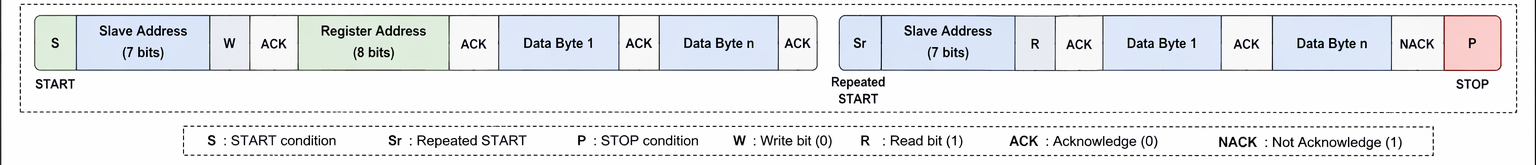
\includegraphics[width=0.9\textwidth]{Figures/i2c_frame.png}
\caption{I2C frame format}
\label{fig:i2c_frame}
\end{figure}

\hspace{1cm}In this project, the I2C interface of the STM32G474MBTx is configured using the HAL library generated by STM32CubeMX. It is used to communicate with external peripherals such as sensors and low-speed devices. The implementation relies on interrupt or polling-based data transfers depending on timing constraints. Particular attention is given to bus stability, including proper pull-up resistor sizing and handling of potential communication errors such as bus busy states or missing acknowledgments.

As shown in Figure~\ref{fig:i2c_bus}, the I2C bus allows multiple slave devices.

\begin{figure}[h]
\centering
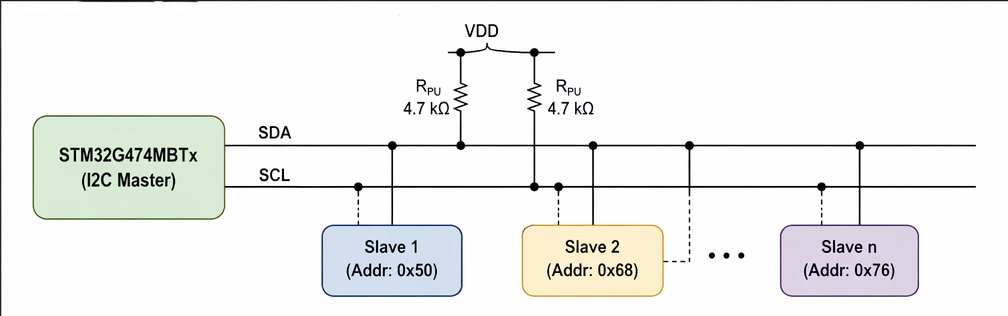
\includegraphics[width=0.6\textwidth]{Figures/i2c_bus.png}
\caption{I2C communication bus architecture}
\label{fig:i2c_bus}
\end{figure}

\subsection{SPI Protocol}


\subsection{UART Protocol}
\hspace{1cm}Universal Asynchronous Receiver-Transmitter (UART) is an asynchronous serial communication protocol that enables full-duplex data exchange between devices without a shared clock signal. Data is transmitted over two lines: Transmit (TX) and Receive (RX). Synchronization between devices is achieved by configuring identical communication parameters, including baud rate, data bits, parity, and stop bits.

\hspace{1cm}Each data frame typically consists of a start bit, followed by a configurable number of data bits (usually 8), an optional parity bit for error detection, and one or more stop bits. Unlike synchronous protocols, UART does not include a clock line, making it simpler but more sensitive to timing mismatches.

\hspace{1cm}In this project, UART is used for communication between the STM32 microcontroller and external systems such as a host computer or other embedded modules. It plays a key role in debugging, logging, and real-time data exchange. The implementation uses the STM32 HAL drivers with support for interrupt-driven and DMA-based transmission to ensure efficient and non-blocking communication. Error handling mechanisms, including overrun, framing, and noise errors, are also considered to improve communication reliability.

The UART frame structure is illustrated in Figure~\ref{fig:uart_frame}.

\begin{figure}[h]
\centering
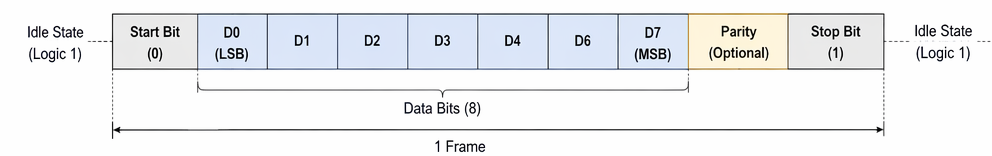
\includegraphics[width=0.9\textwidth]{Figures/uart_frame.png}
\caption{UART frame format}
\label{fig:uart_frame}
\end{figure}


\subsection{RS485 Communication}
\hspace{1cm}RS485 is a robust differential serial communication standard widely used in industrial environments due to its high noise immunity and long-distance capabilities. Unlike single-ended UART communication, RS485 transmits data over a differential pair of lines (A and B), where the information is encoded as a voltage difference between the two conductors. This approach significantly reduces susceptibility to electromagnetic interference and ground potential differences.

\hspace{1cm}The RS485 standard supports half-duplex communication in multi-drop configurations, allowing multiple nodes to share the same bus. However, only one device can transmit at a time, which requires proper bus arbitration at the software level or through protocol design.

\hspace{1cm}In this project, RS485 communication is implemented using the UART peripheral of the STM32G474MBTx combined with an external RS485 transceiver. The transceiver converts TTL-level UART signals into differential signals suitable for the bus. A dedicated GPIO pin is used to control the Driver Enable (DE) and Receiver Enable (RE) pins of the transceiver, allowing the system to switch between transmission and reception modes.

\hspace{1cm}Before transmission, the microcontroller sets the DE pin high to enable the driver stage. After sending the data frame, the DE pin is reset to return the transceiver to reception mode. This timing control is critical to avoid bus contention. The communication is typically used for reliable data exchange in noisy environments, especially when longer cable lengths are required compared to standard UART.

Figure~\ref{fig:rs485_bus} illustrates a typical RS485 bus configuration.

\begin{figure}[h]
\centering
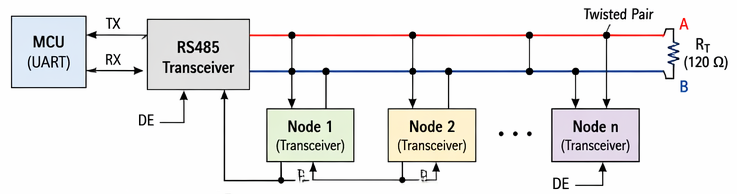
\includegraphics[width=0.65\textwidth]{Figures/rs485_bus.png}
\caption{RS485 differential bus with multi-node configuration}
\label{fig:rs485_bus}
\end{figure}

\subsection{LIN Protocol}
\hspace{1cm}\nobreak{}
Local Interconnect Network (LIN) is a low-cost serial communication protocol designed for distributed control systems, particularly in automotive applications. It operates on a single-wire physical layer and follows a strict master-slave architecture where the master node controls the entire bus communication schedule.

\hspace{1cm}Unlike event-driven protocols, LIN is time-triggered, meaning communication is organized into predefined frames sent at fixed intervals. Each frame consists of a header transmitted by the master and a response transmitted by a slave node. The header includes a break field (used to signal the start of a frame), a synchronization byte, and an identifier field that determines which node should respond.

\hspace{1cm}The data response typically contains up to 8 bytes, followed by a checksum used for error detection. LIN achieves deterministic timing by enforcing strict scheduling, making it suitable for non-critical but predictable control tasks.

\hspace{1cm}In this project, LIN communication is implemented using the STM32 UART peripheral configured in LIN mode. The hardware support simplifies break detection and synchronization field handling, reducing software complexity. The system can therefore reliably detect frame boundaries and process incoming data with minimal CPU overhead.

The LIN frame structure is shown in Figure~\ref{fig:lin_frame}.

\begin{figure}[h]
\centering

\includegraphics[width=0.7\textwidth]{Figures/lin_frame.png}
\caption{LIN frame structure}
\label{fig:lin_frame}
\end{figure}

\subsection{CAN Protocol}

\subsection{Digital-to-Analog Converter (DAC)}
\hspace{1cm}The Digital-to-Analog Converter (DAC) is an analog output peripheral integrated within the STM32G474MBTx microcontroller. It converts digital values stored in memory into continuous analog voltage levels with a resolution defined by the DAC bit width. This allows the generation of precise voltage references or analog waveforms such as sine waves, ramps, or arbitrary signals.

\hspace{1cm}The DAC can operate in several modes, including software-triggered mode, timer-triggered mode, and DMA-driven mode. In timer-triggered mode, a hardware timer periodically updates the DAC output, ensuring precise and deterministic signal timing. When combined with Direct Memory Access (DMA), the DAC can continuously output precomputed waveform data without CPU intervention, significantly improving efficiency.

\hspace{1cm}In this project, the DAC is used for controlled analog signal generation required for system-level testing and control purposes. Its integration with timers ensures synchronization with other system events, enabling deterministic behavior in real-time applications. This is particularly useful in embedded control systems where stable analog references or periodic waveforms are required.

An example of DAC signal generation is illustrated in Figure~\ref{fig:dac_waveform}.

\begin{figure}[h]
\centering
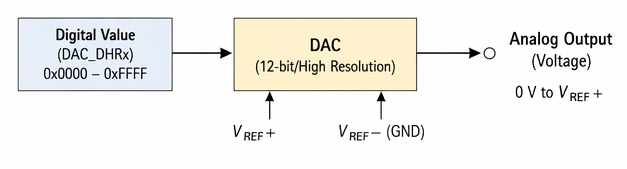
\includegraphics[width=0.5\textwidth]{Figures/dac_waveform.png}
\caption{Example of analog signal generated by DAC}
\label{fig:dac_waveform}
\end{figure}

\subsection{Analog-to-Digital Converter (ADC)}

